\documentclass[a4paper]{article}
\usepackage{student}
\usepackage{graphicx}
\usepackage{caption}
\usepackage[version=4]{mhchem}
\usepackage{tikz}
\usetikzlibrary{shapes.geometric, arrows.meta, positioning, decorations.pathreplacing}
\usepackage{enumitem}
\usepackage{amsmath}
\usepackage{tikz-3dplot}
\usepackage{booktabs}
\usepackage[table]{xcolor}
\usepackage{caption}
\tikzstyle{arrow} = [thick,->,>=stealth]

% Definindo o estilo de destaque com linhas pontilhadas
\tikzstyle{highlight} = [draw, dashed, thick, rectangle, rounded corners, inner sep=0.2cm, orange]


\tikzstyle{startstop} = [
rectangle, rounded corners, minimum width=0.5cm,
text centered, draw=black, fill=blue!10, font=\small
]
\tikzstyle{startstop_S} = [
rectangle, rounded corners, minimum width=0.5cm, minimum height=0.8cm,
text centered, draw=black, fill=green!30, font=\small
]
\tikzstyle{decision} = [
diamond, aspect=2, draw=black, fill=orange!15, align=center,
text centered, inner sep=0pt, font=\small
]
\tikzstyle{decision_S} = [
diamond, aspect=2, draw=black, fill=orange!30, align=center,
text centered, inner sep=0pt, font=\small
]
\tikzstyle{arrow} = [thick,->,>=stealth]



% Metadata
\date{\today}
\setmodule{PGF5261/IFUSP: Teoria de Grupos Aplicada a Sólidos e Moléculas. Prof.: Lucy Assali} 
\setterm{1o. semestre, 2025}

%-------------------------------%
% Other details
% TODO: Fill these
%-------------------------------%
\title{Exercício 03 - 13/05}
\setmembername{Nara Avila Moraes}  % Fill group member names
\setmemberuid{5716734}  % Fill group member uids (same order)

%-------------------------------%
% Add / Delete commands and packages
% TODO: Add / Delete here as you need
%-------------------------------%
\usepackage{amsmath,amssymb,bm}

\newcommand{\KL}{\mathrm{KL}}
\newcommand{\R}{\mathbb{R}}
\newcommand{\E}{\mathbb{E}}
\newcommand{\T}{\top}

\newcommand{\expdist}[2]{%
\normalfont{\textsc{Exp}}(#1, #2)%
}
\newcommand{\expparam}{\bm \lambda}
\newcommand{\Expparam}{\bm \Lambda}
\newcommand{\natparam}{\bm \eta}
\newcommand{\Natparam}{\bm H}
\newcommand{\sufstat}{\bm u}

% Main document
\begin{document}
% Add header
\header{}

\textbf{Questão 1.}
Considere as simetrias e a ligaçâo \(\pi\)  da molécula de benzeno  \ce{C6H6} e responda os seguintes ítems:

\begin{center}
	\begin{minipage}{0.25\textwidth}
		\centering
		\includegraphics[width=0.8\textwidth]{figuras/benzeno1.png}  % Substitua pelo nome correto do arquivo
		\captionof{figure}{Ligaçôes \(\sigma\) no plano da molécula}
	\end{minipage}
	\hfill
        \begin{minipage}{0.25\textwidth}
		\centering
		\includegraphics[width=0.8\textwidth]{figuras/benzeno2.png}  % Substitua pelo nome correto do arquivo
		\captionof{figure}{Orbitais \(p_z\) perpendiculares ao plano da molécula}
	\end{minipage}
	\hfill
        \begin{minipage}{0.45\textwidth}
		\centering
		\includegraphics[width=0.8\textwidth]{figuras/benzeno3.png}  % Substitua pelo nome correto do arquivo
		\captionof{figure}{Ligação \(\pi\) do \ce{C6H6}}
	\end{minipage}
	\hfill
        \begin{itemize}
            \item[(1.1)] Encontre o grupo de simetria da molécula (descrição das operações ou desenho).
            \item[(1.2)] Dados os orbitais \(p_z\) dos seis átomos de carbono que formam os orbitais moleculares \(\pi\), encontrar a representação \(\Gamma_{pz}^{\pi}\) \(\implies\) traços das matrizes dos operadores de transformação dos orbitais \(p_z\) (\(\varphi_1, \varphi_2, \varphi_3, \varphi_4, \varphi_5, \varphi_6\))
            \item[(1.3)] Encontre as representaçôes irredutíveis do grupo da molécula às quais os orbitais \(p_z\) se transformam.
            \item[(1.4)] Obter os orbitais \(\pi\) simetrizados (e normalizados) da molécula \(\implies\) Aplicar os operadores de projeçâo para obter as funções projetadas nos subespaços das representações irredutíveis.
            \item[(1.5)] Obter as energiais orbitais (Hückel) das ligações \(\pi\) (fatoração da equação secular)
        \end{itemize}

\end{center}

\begin{answer}[Ítem 1.1 - Grupo de Simetria da Molécula]
\begin{itemize}[noitemsep, topsep=0pt, label={}, leftmargin=0pt]

\item \noindent\parbox[t]{\linewidth}{A molécula \ce{C6H6} contem as seguintes simetrias: \\}
%%%%%%%%%%%%%%%%%%%%%%%%%%%%%%%%%%%%%%%%%%%%%%%%%%%%%%%%%%%%%%%%%%%%%%%% 
%                                  E
%%%%%%%%%%%%%%%%%%%%%%%%%%%%%%%%%%%%%%%%%%%%%%%%%%%%%%%%%%%%%%%%%%%%%%%% 		      
\begin{minipage}[t]{0.48\textwidth}
			      \centering
			      \includegraphics[width=0.6\linewidth]{figuras/E.png}
			      \captionof{figure}{Simetria \(E\)}
		      \end{minipage}
		      \hfill
		      \begin{minipage}[t]{0.48\textwidth}
			      \centering
			      \includegraphics[width=0.6\linewidth]{figuras/E.png}
			      \captionof{figure}{Operação \( E \) aplicada}
		      \end{minipage}
         \begin{align*}
        \textbf{Identidade (\(E\)):}\quad & E(1,2,3,4,5,6) = (1,2,3,4,5,6)
        \end{align*}

%%%%%%%%%%%%%%%%%%%%%%%%%%%%%%%%%%%%%%%%%%%%%%%%%%%%%%%%%%%%%%%%%%%%%%%% 
%                                  C6 
%%%%%%%%%%%%%%%%%%%%%%%%%%%%%%%%%%%%%%%%%%%%%%%%%%%%%%%%%%%%%%%%%%%%%%%% 
        \begin{minipage}[t]{0.48\textwidth}
			      \centering
			      \includegraphics[width=0.6\linewidth]{figuras/C6.png}
			      \captionof{figure}{Eixo de rotação \(C_6\)}
		      \end{minipage}
		      \hfill
		      \begin{minipage}[t]{0.48\textwidth}
			      \centering
			      \includegraphics[width=0.6\linewidth]{figuras/C6_1.png}
			      \captionof{figure}{Operação \( C_6^{+} \) aplicada}
		      \end{minipage}
\begin{align*}
\textbf{Rotações próprias (\(C_6^{\pm}\)):}\quad
& C_6^{+}\,(1,2,3,4,5,6) = (6,1,2,3,4,5), \\
& C_6^{-}\,(1,2,3,4,5,6)   = (2,3,4,5,6,1)
\end{align*}

%%%%%%%%%%%%%%%%%%%%%%%%%%%%%%%%%%%%%%%%%%%%%%%%%%%%%%%%%%%%%%%%%%%%%%%% 
%                                  C3
%%%%%%%%%%%%%%%%%%%%%%%%%%%%%%%%%%%%%%%%%%%%%%%%%%%%%%%%%%%%%%%%%%%%%%%% 
        \begin{minipage}[t]{0.48\textwidth}
			      \centering
			      \includegraphics[width=0.6\linewidth]{figuras/C6.png}
			      \captionof{figure}{Eixo de rotação \(C_3\)}
		      \end{minipage}
		      \hfill
		      \begin{minipage}[t]{0.48\textwidth}
			      \centering
			      \includegraphics[width=0.6\linewidth]{figuras/C3_1.png}
			      \captionof{figure}{Operação \( C_3^{+} \) aplicada}
		      \end{minipage}
\begin{align*}
\textbf{Rotações próprias (\(C_3^{\pm}\)):}\quad
& C_3^{+}\,(1,2,3,4,5,6) = (5,6,1,2,3,4),\\
& C_3^{-}\,(1,2,3,4,5,6) = (3,4,5,6,1,2)
\end{align*}
%%%%%%%%%%%%%%%%%%%%%%%%%%%%%%%%%%%%%%%%%%%%%%%%%%%%%%%%%%%%%%%%%%%%%%%% 
%                                  C2
%%%%%%%%%%%%%%%%%%%%%%%%%%%%%%%%%%%%%%%%%%%%%%%%%%%%%%%%%%%%%%%%%%%%%%%% 
        \begin{minipage}[t]{0.48\textwidth}
			      \centering
			      \includegraphics[width=0.6\linewidth]{figuras/C6.png}
			      \captionof{figure}{Eixo de rotação \(C_2\)}
		      \end{minipage}
		      \hfill
		      \begin{minipage}[t]{0.48\textwidth}
			      \centering
			      \includegraphics[width=0.6\linewidth]{figuras/C2_1.png}
			      \captionof{figure}{Operação \( C_2^{\pm} \) aplicada}
		      \end{minipage}
\begin{align*}
\textbf{Rotação própria (\(C_2^{\pm}\)):}\quad
& C_2^{\pm}\,(1,2,3,4,5,6) = (4,5,6,1,2,3)
\end{align*}
%%%%%%%%%%%%%%%%%%%%%%%%%%%%%%%%%%%%%%%%%%%%%%%%%%%%%%%%%%%%%%%%%%%%%%%% 
%                                  C2'
%%%%%%%%%%%%%%%%%%%%%%%%%%%%%%%%%%%%%%%%%%%%%%%%%%%%%%%%%%%%%%%%%%%%%%%% 
        \begin{minipage}[t]{0.48\textwidth}
			      \centering
			      \includegraphics[width=0.6\linewidth]{figuras/C2'.png}
			      \captionof{figure}{Eixo de rotação \(C_{2}'^{(1)}\)}
		      \end{minipage}
		      \hfill
		      \begin{minipage}[t]{0.48\textwidth}
			      \centering
			      \includegraphics[width=0.6\linewidth]{figuras/C2'_1.png}
			      \captionof{figure}{Operação \(C_{2}'^{(1)}\) aplicada}
		      \end{minipage}
\begin{align*}
\textbf{Rotação (\(C_{2}^{'(k)}\)):}\quad
& C_{2}'^{(1)}\,(1,2,3,4,5,6) = (1,6,5,4,3,2),\\
& C_{2}'^{(2)}\,(1,2,3,4,5,6) = (3,2,1,6,5,4),\\
& C_{2}'^{(3)}\,(1,2,3,4,5,6) = (5,4,3,2,1,6)
\end{align*}

%%%%%%%%%%%%%%%%%%%%%%%%%%%%%%%%%%%%%%%%%%%%%%%%%%%%%%%%%%%%%%%%%%%%%%%% 
%                                  C2''
%%%%%%%%%%%%%%%%%%%%%%%%%%%%%%%%%%%%%%%%%%%%%%%%%%%%%%%%%%%%%%%%%%%%%%%% 
        \begin{minipage}[t]{0.48\textwidth}
			      \centering
			      \includegraphics[width=0.6\linewidth]{figuras/C2''.png}
			      \captionof{figure}{Eixo de rotação \(C_{2}''^{(1)}\)}
		      \end{minipage}
		      \hfill
		      \begin{minipage}[t]{0.48\textwidth}
			      \centering
			      \includegraphics[width=0.6\linewidth]{figuras/C2''_1.png}
			      \captionof{figure}{Operação \(C_{2}''^{(1)}\) aplicada}
		      \end{minipage}
\begin{align*}
\textbf{Rotação (\(C_{2}''^{(k)}\)):}\quad
& C_{2}''^{(1)}\,(1,2,3,4,5,6) = (2,1,6,5,4,3),\\
& C_{2}''^{(2)}\,(1,2,3,4,5,6) = (4,3,2,1,6,5),\\
& C_{2}''^{(3)}\,(1,2,3,4,5,6) = (6,5,4,3,2,1)
\end{align*}

%%%%%%%%%%%%%%%%%%%%%%%%%%%%%%%%%%%%%%%%%%%%%%%%%%%%%%%%%%%%%%%%%%%%%%%% 
%                                  i
%%%%%%%%%%%%%%%%%%%%%%%%%%%%%%%%%%%%%%%%%%%%%%%%%%%%%%%%%%%%%%%%%%%%%%%% 
                \begin{minipage}[t]{0.48\textwidth}
			      \centering
			      \includegraphics[width=0.6\linewidth]{figuras/Ci.png}
			      \captionof{figure}{Origem da inversão \(i\)}
		      \end{minipage}
		      \hfill
		      \begin{minipage}[t]{0.48\textwidth}
			      \centering
			      \includegraphics[width=0.6\linewidth]{figuras/Ci_1.png}
			      \captionof{figure}{Operação inversão \(i\) aplicada}
		      \end{minipage}
\begin{align*}
\textbf{Inversão (\(i\)):}\quad
& i(1,2,3,4,5,6) = (4,5,6,1,2,3)
\end{align*}

%%%%%%%%%%%%%%%%%%%%%%%%%%%%%%%%%%%%%%%%%%%%%%%%%%%%%%%%%%%%%%%%%%%%%%%% 
%                                  S3
%%%%%%%%%%%%%%%%%%%%%%%%%%%%%%%%%%%%%%%%%%%%%%%%%%%%%%%%%%%%%%%%%%%%%%%% 
        \begin{minipage}[t]{0.31\textwidth}
			      \centering
			      \includegraphics[width=0.6\linewidth]{figuras/C6.png}
			      \captionof{figure}{Eixo de rotação \(C_{3}^{+}\)}
		      \end{minipage}
		      \hfill
		      \begin{minipage}[t]{0.31\textwidth}
			      \centering
			      \includegraphics[width=0.6\linewidth]{figuras/sigma_h.png}
			      \captionof{figure}{Plano de reflexão \(\sigma_{h} \) }
		      \end{minipage}
              \begin{minipage}[t]{0.31\textwidth}
			      \centering
			      \includegraphics[width=0.6\linewidth]{figuras/s3_1.png}
			      \captionof{figure}{Operação \(S_{3}^{+} \) aplicada}
		      \end{minipage}
        \begin{align*}\textbf{Rotações Impróprias ( \( S_{3}^{\pm}\)):} \quad 
& S_3^{+} = \sigma_h\circ C_3^{+}:\;(1,2,3,4,5,6)\xrightarrow{C_3^{+}}(5,6,1,2,3,4)\xrightarrow{\sigma_h}(5,6,1,2,3,4),\\
& S_3^{-} = \sigma_h\circ C_3^{-}:\;(1,2,3,4,5,6)\xrightarrow{C_3^{-}}(3,4,5,6,1,2)\xrightarrow{\sigma_h}(3,4,5,6,1,2)
\end{align*}

%%%%%%%%%%%%%%%%%%%%%%%%%%%%%%%%%%%%%%%%%%%%%%%%%%%%%%%%%%%%%%%%%%%%%%%% 
%                                  S6
%%%%%%%%%%%%%%%%%%%%%%%%%%%%%%%%%%%%%%%%%%%%%%%%%%%%%%%%%%%%%%%%%%%%%%%% 
        \begin{minipage}[t]{0.31\textwidth}
			      \centering
			      \includegraphics[width=0.6\linewidth]{figuras/C6.png}
			      \captionof{figure}{Eixo de rotação \(C_{6}^{+}\)}
		      \end{minipage}
		      \hfill
		      \begin{minipage}[t]{0.31\textwidth}
			      \centering
			      \includegraphics[width=0.6\linewidth]{figuras/sigma_h.png}
			      \captionof{figure}{Plano de reflexão \(\sigma_{h} \) }
		      \end{minipage}
              \begin{minipage}[t]{0.31\textwidth}
			      \centering
			      \includegraphics[width=0.6\linewidth]{figuras/S6_1.png}
			      \captionof{figure}{Operação \(S_{6}^{+} \) aplicada}
		      \end{minipage}
        \begin{align*}\textbf{Rotações Impróprias ( \( S_{6}^{\pm}\)):} \quad 
& S_6^{+} = \sigma_h\circ C_6^{+}:\;(1,2,3,4,5,6)\xrightarrow{C_6^{+}}(6,1,2,3,4,5)\xrightarrow{\sigma_h}(6,1,2,3,4,5),\\
& S_6^{-} = \sigma_h\circ C_6^{-}:\;(1,2,3,4,5,6)\xrightarrow{C_6^{-}}(2,3,4,5,6,1)\xrightarrow{\sigma_h}(2,3,4,5,6,1)
\end{align*}

%%%%%%%%%%%%%%%%%%%%%%%%%%%%%%%%%%%%%%%%%%%%%%%%%%%%%%%%%%%%%%%%%%%%%%%% 
%                                  sigma h
%%%%%%%%%%%%%%%%%%%%%%%%%%%%%%%%%%%%%%%%%%%%%%%%%%%%%%%%%%%%%%%%%%%%%%%% 
                \begin{minipage}[t]{0.48\textwidth}
			      \centering
			      \includegraphics[width=0.6\linewidth]{figuras/sigma_h.png}
			      \captionof{figure}{Plano de reflexão \(\sigma_{h}\)}
		      \end{minipage}
		      \hfill
		      \begin{minipage}[t]{0.48\textwidth}
			      \centering
			      \includegraphics[width=0.6\linewidth]{figuras/E.png}
			      \captionof{figure}{Operação \(\sigma_{h} \) aplicada}
		      \end{minipage}
              
\begin{align*}
\textbf{Reflexão horizontal (\(\sigma_{h}\)):}\quad
& \sigma_h\,(1,2,3,4,5,6) = (1,2,3,4,5,6)
\end{align*}

%%%%%%%%%%%%%%%%%%%%%%%%%%%%%%%%%%%%%%%%%%%%%%%%%%%%%%%%%%%%%%%%%%%%%%%% 
%                                  sigma d
%%%%%%%%%%%%%%%%%%%%%%%%%%%%%%%%%%%%%%%%%%%%%%%%%%%%%%%%%%%%%%%%%%%%%%%% 
                \begin{minipage}[t]{0.48\textwidth}
			      \centering
			      \includegraphics[width=0.6\linewidth]{figuras/sigma_d.png}
			      \captionof{figure}{Plano de reflexão \(\sigma_{d}^{(1)}\)}
		      \end{minipage}
		      \hfill
		      \begin{minipage}[t]{0.48\textwidth}
			      \centering
			      \includegraphics[width=0.6\linewidth]{figuras/sigma_d_1.png}
			      \captionof{figure}{Operação \(\sigma_{d}^{(1)} \) aplicada}
		      \end{minipage}
              
\begin{align*}
\textbf{Reflexões diagonais (\(\sigma_{d}^{(k)}\)):}\quad
& \sigma_{d}^{(1)}\,(1,2,3,4,5,6) = (4,3,2,1,6,5),\\
& \sigma_{d}^{(2)}\,(1,2,3,4,5,6) = (2,1,6,5,4,3),\\
& \sigma_{d}^{(3)}\,(1,2,3,4,5,6) = (6,5,4,3,2,1)
\end{align*}
%%%%%%%%%%%%%%%%%%%%%%%%%%%%%%%%%%%%%%%%%%%%%%%%%%%%%%%%%%%%%%%%%%%%%%%% 
%                                  sigma v
%%%%%%%%%%%%%%%%%%%%%%%%%%%%%%%%%%%%%%%%%%%%%%%%%%%%%%%%%%%%%%%%%%%%%%%% 
        \begin{minipage}[t]{0.48\textwidth}
			      \centering
			      \includegraphics[width=0.6\linewidth]{figuras/sigma_v.png}
			      \captionof{figure}{Plano de reflexão \(\sigma_{v}^{(1)}\)}
		      \end{minipage}
		      \hfill
		      \begin{minipage}[t]{0.48\textwidth}
			      \centering
			      \includegraphics[width=0.6\linewidth]{figuras/sigma_v_1.png}
			      \captionof{figure}{Operação \(\sigma_{v}^{(1)} \) aplicada}
		      \end{minipage}
        \begin{align*}
        \textbf{Reflexões verticais (\(\sigma_{v}^{k}\)):}\quad   & \sigma_{v}^{(1)}\,(1,2,3,4,5,6) = (5,4,3,2,1,6),\\
        & \sigma_{v}^{(2)}\,(1,2,3,4,5,6) = (3,2,1,6,5,4),\\
        & \sigma_{v}^{(3)}\,(1,2,3,4,5,6) = (1,6,5,4,3,2)
        \end{align*}

Portanto, analisando as simetrias encontradas, conforme podemos confirmar pelo fluxograma, com \(n = 6\) o grupo de simetria da molécula de benzeno é o \(D_{6h}\).
\\
	\begin{center}
		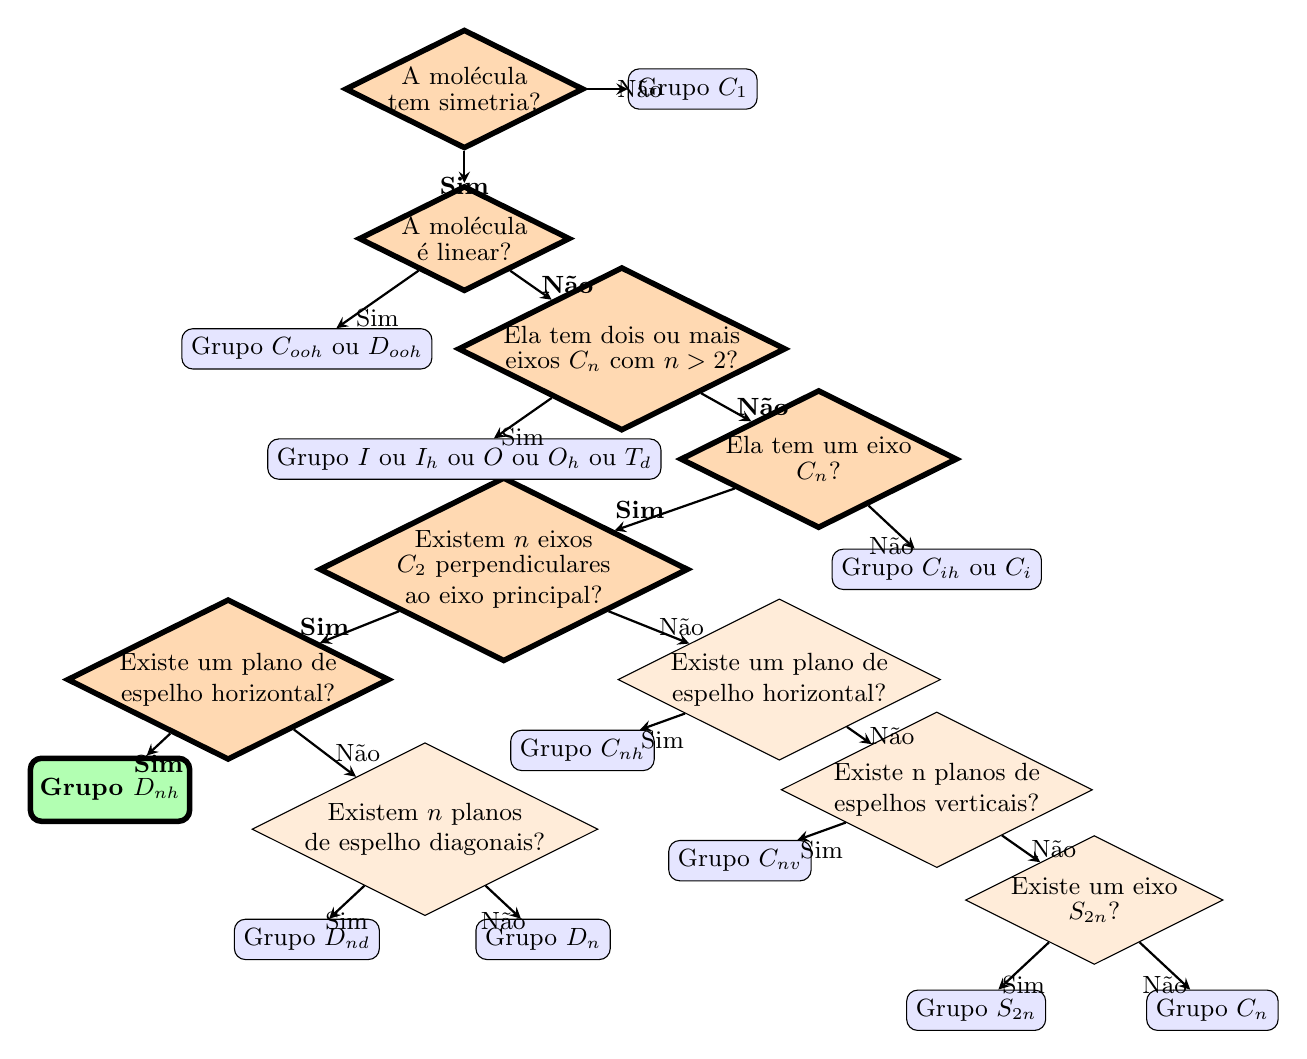
\begin{tikzpicture}[node distance=1.4cm]
			% Definindo as 15 decisões
			\node (Q_1) [decision_S, xshift=-7cm, line width=0.7mm] {\shortstack{A molécula\\tem simetria?}};
			\node (Q_2) [decision_S, below of=Q_1, yshift=-0.5cm, line width=0.7mm] {\shortstack{A molécula\\é linear?}};
			\node (Q_4) [decision_S, below of=Q_2, xshift=2cm, line width=0.7mm] {\shortstack{Ela tem dois ou mais\\eixos \( C_n \) com \( n>2 \)?}};
			\node (Q_6) [decision_S, below of=Q_4, xshift=2.5cm, line width=0.7mm] {\shortstack{Ela tem um eixo\\\( C_n \)?}};
			\node (Q_9) [decision_S, below of=Q_6, xshift=-4cm, line width=0.7mm] {\shortstack{Existem \( n \) eixos\\\( C_2 \) perpendiculares\\ao eixo principal?}};
			\node (Q_10) [decision_S, below of=Q_9, xshift=-3.5cm, line width=0.7mm] {\shortstack{Existe um plano de\\espelho horizontal?}};
			\node (Q_11) [decision, below of=Q_10, xshift=2.5cm, yshift=-0.5cm] {\shortstack{Existem \( n \) planos\\de espelho diagonais?}};
			\node (Q_12) [decision, below of=Q_9, xshift=3.5cm] {\shortstack{Existe um plano de\\espelho horizontal?}};
			\node (Q_13) [decision, below of=Q_12, xshift=2cm] {\shortstack{Existe n planos de\\espelhos verticais?}};
			\node (Q_14) [decision, below of=Q_13, xshift=2cm] {\shortstack{Existe um eixo\\\( S_{2n} \)?}};

			% Caminhos
			\node (CooDoo) [startstop, below of=Q_2, xshift=-2cm] {Grupo $C_{ooh}$ ou $D_{ooh}$};
			\node (G_alta_simetria) [startstop, below of=Q_4, xshift=-2cm] {Grupo $I$ ou $I_h$ ou $O$ ou $O_h$ ou $T_d$};
			\node (G_baixa_simetria) [startstop, below of=Q_6, xshift=1.5cm] {Grupo $C_{ih}$ ou $C_i$};
			\node (Dnh) [startstop_S, below of=Q_10, xshift=-1.5cm, line width=0.7mm] {\textbf{Grupo $D_{nh}$}};
			\node (Dnd) [startstop, below of=Q_11, xshift=-1.5cm] {Grupo $D_{nd}$};
			\node (Dn) [startstop, below of=Q_11, xshift=1.5cm] {Grupo $D_n$};
			\node (Cnv) [startstop, below of=Q_13, xshift=-2.5cm, yshift=0.5cm] {Grupo $C_{nv}$};
			\node (Cnh) [startstop, below of=Q_12, xshift=-2.5cm, yshift=0.5cm] {Grupo $C_{nh}$};
			\node (S2n) [startstop, below of=Q_14, xshift=-1.5cm] {Grupo $S_{2n}$};
			\node (Cn) [startstop, below of=Q_14, xshift=1.5cm] {Grupo $C_n$};
			\node (C1) [startstop, right of=Q_1, xshift=1.5cm] {Grupo $C_1$};

			% Connections
			\draw [arrow] (Q_1) -- node[anchor=north, font=\small] {\textbf{Sim}} (Q_2);
			\draw [arrow] (Q_2) -- node[anchor=west, font=\small] {\textbf{Não}} (Q_4);
			\draw [arrow] (Q_4) -- node[anchor=west, font=\small] {\textbf{Não}} (Q_6);
			\draw [arrow] (Q_6) -- node[anchor=east, font=\small] {\textbf{Sim}} (Q_9);
			\draw [arrow] (Q_9) -- node[anchor=east, font=\small] {\textbf{Sim}} (Q_10);
			\draw [arrow] (Q_10) -- node[anchor=west, font=\small] {Não} (Q_11);
			\draw [arrow] (Q_9) -- node[anchor=west, font=\small] {Não} (Q_12);
			\draw [arrow] (Q_12) -- node[anchor=west, font=\small] {Não} (Q_13);
			\draw [arrow] (Q_13) -- node[anchor=west, font=\small] {Não} (Q_14);

			% Final Connections
			\draw [arrow] (Q_2) -- node[anchor=north, font=\small] {Sim} (CooDoo);
			\draw [arrow] (Q_4) -- node[anchor=north, font=\small] {Sim} (G_alta_simetria);
			\draw [arrow] (Q_6) -- node[anchor=north, font=\small] {Não} (G_baixa_simetria);
			\draw [arrow] (Q_10) -- node[anchor=north, font=\small] {\textbf{Sim}} (Dnh);
			\draw [arrow] (Q_11) -- node[anchor=north, font=\small] {Sim} (Dnd);
			\draw [arrow] (Q_11) -- node[anchor=north, font=\small] {Não} (Dn);
			\draw [arrow] (Q_12) -- node[anchor=north, font=\small] {Sim} (Cnh);
			\draw [arrow] (Q_13) -- node[anchor=north, font=\small] {Sim} (Cnv);
			\draw [arrow] (Q_14) -- node[anchor=north, font=\small] {Sim} (S2n);
			\draw [arrow] (Q_14) -- node[anchor=north, font=\small] {Não} (Cn);
			\draw [arrow] (Q_1) -- node[anchor=west, font=\small] {Não} (C1);

		\end{tikzpicture}
	\end{center}
        
	\end{itemize}
\end{answer}

\begin{answer}[Ítem 1.2 - A representação \(\Gamma_{pz}^{\pi}\)]
Para encontrar o traço das matrizes dos operadores de transformação dos orbitais \(p_z\), isto é \(\varphi_1\), \(\varphi_2\), \(\varphi_3\), \(\varphi_4\), \(\varphi_5\), \(\varphi_6\) na Figura 2, não precisamos necessariamente escolher uma base e descrever as operações de simetria do grupo \(D_{6h}\) na forma matricial. Isto porque o traço destas matrizes será invariante independente da base. Podemos fazer uma análise posicional de acordo com a transformação aplicada, da seguinte forma: verificamos se ao aplicar a transformação cada orbital \(\varphi_i\) manteve-se no mesmo sítio, se sim, este orbital contribuirá com valor +1 para o traço caso não tenha havido inversão de polaridade, e -1 caso tenha havido, e 0 caso tenha se deslocado do seu sítio original, isto porque apenas os valores da diagonal contribuem para o traço e um deslocamento significa que a sua posição original terá contribuição nula no resultado da transformação. Além disso, só precisamos verificar o traço de uma transformação de cada classe, uma vez que dentro de uma mesma classe o traço não varia.

As classes do grupo de simetria \(D_{6h}\) são:
\[
\{E\},\,\{C_6, C_6^{-1}\},\,\{C_3, C_3^{-1}\},\,\{C_2\},\,\{3C_2'\},\,\{3C_2''\},\,\{i\},\,\{S_3, S_3^{-1}\},\,\{S_6, S_6^{-1}\},\,\{\sigma_h\},\,\{3\sigma_v\},\,\{3\sigma_d\}
\]

Com base nas permutações analisadas no ítem 1.1, obtemos os seguintes traços das matrizes de transformação de cada classe:
\vspace{-1.4em}
\begin{flushleft}
\[
\setlength{\arraycolsep}{0pt} 
\begin{array}{r@{\hskip 0.2em}l}
\chi^{\Gamma_{pz}}(E) &= \text{Todos os orbitais permanecem no lugar com mesma polaridade } \Rightarrow 6 \\
\chi^{\Gamma_{pz}}(2C_6) &= \text{Ex: } C_6^+(1,2,3,4,5,6) = (2,3,4,5,6,1) \Rightarrow 0\\
\chi^{\Gamma_{pz}}(2C_3) &= \text{Ex: } C_3^+(1,2,3,4,5,6) = (3,4,5,6,1,2) \Rightarrow 0\\
\chi^{\Gamma_{pz}}(C_2) &= \text{Ex: } C_2(1,2,3,4,5,6) = (4,5,6,1,2,3) \Rightarrow 0\\
\chi^{\Gamma_{pz}}(3C_2') &= \text{Ex: } C_2^{\prime(1)}(1,2,3,4,5,6) = (1,6,5,4,3,2) \Rightarrow -2\\
\chi^{\Gamma_{pz}}(3C_2'') &= \text{Ex: } C_2^{\prime\prime(1)}(1,2,3,4,5,6) = (2,1,6,5,4,3) \Rightarrow 0\\
\chi^{\Gamma_{pz}}(i) &= \text{Inversão: troca todos os sítios e inverte polaridade} \Rightarrow 0\\
\chi^{\Gamma_{pz}}(2S_3) &= \text{Ex: } S_3^+(1,2,3,4,5,6) = (3,4,5,6,1,2) \Rightarrow 0 \\
\chi^{\Gamma_{pz}}(2S_6) &= \text{Ex: } S_6^+(1,2,3,4,5,6) = (2,3,4,5,6,1) \Rightarrow 0 \\
\end{array}
\]
\end{flushleft}
\begin{flushleft}
\[
\setlength{\arraycolsep}{0pt} 
\begin{array}{r@{\hskip 0.2em}l}
\chi^{\Gamma_{pz}}(\sigma_h) &= \text{Ex: } \sigma_h(1,2,3,4,5,6) = (1,2,3,4,5,6) \Rightarrow -6 \\
\chi^{\Gamma_{pz}}(3\sigma_d) &= \text{Ex: } \sigma_d^{(1)}(1,2,3,4,5,6) = (2,1,6,5,4,3) \Rightarrow 0\\
\chi^{\Gamma_{pz}}(3\sigma_v) &= \text{Ex: } \sigma_v^{(1)}(1,2,3,4,5,6) = (1,6,5,4,3,2) \Rightarrow 2
\end{array}
\]
\end{flushleft}

Portanto estes são os caracteres que compõem a representação \(\Gamma_{pz}^{\pi}\):

\begin{minipage}{\textwidth}
\centering
\vspace{0.5em}
\renewcommand{\arraystretch}{1.4}
\begin{tabular}{c|cccccccccccc}
    \toprule
    Classes & $E$ & $2C_6$ & $2C_3$ & $C_2$ & $3C_2'$ & $3C_2''$ & $i$ & $2S_3$ & $2S_6$ & $\sigma_h$ & $3\sigma_d$ & $3\sigma_v$ \\
    \midrule
    $\Gamma_{pz}^{\pi}$ & 6 & 0 & 0 & 0 & -2 & 0 & 0 & 0 & 0 & -6 & 0 & 2 \\
    \bottomrule
\end{tabular}
\captionof{table}{A representação \(\Gamma_{pz}^{\pi}\) para o grupo \(D_{6h}\)}
\end{minipage}


\end{answer}

\begin{answer}[Ítem 1.3 - Representações irredutíveis aos quais os orbitais \(p_z\) se transformam]

Com base na tabela de caracteres do grupo de simetria \(D_{6h}\), precisamos encontrar os coeficientes de cada representação irredutível na composição de \(\Gamma^{\pi}_{pz}\) sumarizados na seguinte expressão:

\[
n_\alpha \;=\;\frac{1}{h}\sum_{\mu=1}^{p}N_{\mu}\,\chi^{\alpha}(C_{\mu})\,\chi^{\Gamma}(C_{\mu}),
\]

na qual \(h\) é a ordem do grupo (\(h=24\) para \(D_{6h}\)), \(p\) é o número de classes de simetria, e \(N_\mu\) é o número de elementos na \(\mu\)-ésima classe \(C_\mu\). \(\chi^\Gamma(C_\mu)\) e \(\chi^\alpha(C_\mu)\) representam, respectivamente, os caracteres da representação \(\Gamma\) (reduzível) e da \(\alpha\)-ésima representação irreduzível na mesma classe. A partir dos cálculos encontramos a combinação linear que compõe \(\Gamma^{\pi}_{pz}\), isto é, as representações irredutíveis nas quais os orbitais \(p_z\) se transformam.

\[
\begin{aligned}
n_{A_{1g}}
&=\frac{1}{24}\Bigl\{
1\cdot1\cdot6
+2\cdot1\cdot0
+2\cdot1\cdot0
+1\cdot1\cdot0
+3\cdot1\cdot(-2)\\[-3pt]
&\quad\;
+3\cdot1\cdot0
+1\cdot1\cdot0
+2\cdot1\cdot0
+2\cdot1\cdot0
+1\cdot1\cdot(-6)
+3\cdot1\cdot0
+3\cdot1\cdot2
\Bigr\}
=0,\\[6pt]
n_{A_{2g}}
&=\frac{1}{24}\Bigl\{
1\cdot1\cdot6
+2\cdot1\cdot0
+2\cdot1\cdot0
+1\cdot1\cdot0
+3\cdot(-1)\cdot(-2)\\[-3pt]
&\quad\;
+3\cdot(-1)\cdot0
+1\cdot1\cdot0
+2\cdot1\cdot0
+2\cdot1\cdot0
+1\cdot1\cdot(-6)
+3\cdot(-1)\cdot0
+3\cdot(-1)\cdot2
\Bigr\}
=0,\\[6pt]
n_{B_{1g}}
&=\frac{1}{24}\Bigl\{
1\cdot1\cdot6
+2\cdot(-1)\cdot0
+2\cdot1\cdot0
+1\cdot(-1)\cdot0
+3\cdot1\cdot(-2)\\[-3pt]
&\quad\;
+3\cdot(-1)\cdot0
+1\cdot1\cdot0
+2\cdot(-1)\cdot0
+2\cdot1\cdot0
+1\cdot(-1)\cdot(-6)
+3\cdot1\cdot0
+3\cdot(-1)\cdot2
\Bigr\}
=0,\\[6pt]
n_{B_{2g}}
&=\frac{1}{24}\Bigl\{
1\cdot1\cdot6
+2\cdot(-1)\cdot0
+2\cdot1\cdot0
+1\cdot(-1)\cdot0
+3\cdot(-1)\cdot(-2)\\[-3pt]
&\quad\;
+3\cdot1\cdot0
+1\cdot1\cdot0
+2\cdot(-1)\cdot0
+2\cdot1\cdot0
+1\cdot(-1)\cdot(-6)
+3\cdot1\cdot0
+3\cdot1\cdot2
\Bigr\}
=1,\\[6pt]
n_{E_{1g}}
&=\frac{1}{24}\Bigl\{
1\cdot2\cdot6
+2\cdot1\cdot0
+2\cdot(-1)\cdot0
+1\cdot(-2)\cdot0
+3\cdot0\cdot(-2)\\[-3pt]
&\quad\;
+3\cdot0\cdot0
+1\cdot2\cdot0
+2\cdot1\cdot0
+2\cdot(-1)\cdot0
+1\cdot(-2)\cdot(-6)
+3\cdot0\cdot0
+3\cdot0\cdot2
\Bigr\}
=1,\\[6pt]
n_{E_{2g}}
&=\frac{1}{24}\Bigl\{
1\cdot2\cdot6
+2\cdot(-1)\cdot0
+2\cdot(-1)\cdot0
+1\cdot2\cdot0
+3\cdot0\cdot(-2)\\[-3pt]
&\quad\;
+3\cdot0\cdot0
+1\cdot2\cdot0
+2\cdot(-1)\cdot0
+2\cdot(-1)\cdot0
+1\cdot2\cdot(-6)
+3\cdot0\cdot0
+3\cdot0\cdot2
\Bigr\}
=0, \\[6pt]
n_{A_{1u}}
&= \frac{1}{24}\Bigl\{
1\cdot1\cdot6
+2\cdot1\cdot0
+2\cdot1\cdot0
+1\cdot1\cdot0
+3\cdot1\cdot(-2)
+3\cdot1\cdot0\\[-3pt]
&\quad\;
+1\cdot(-1)\cdot0
+2\cdot(-1)\cdot0
+2\cdot(-1)\cdot0
+1\cdot(-1)\cdot(-6)
+3\cdot(-1)\cdot0
+3\cdot(-1)\cdot2
\Bigr\}
=0,\\[6pt]
\end{aligned}
\]
\[
\begin{aligned}
n_{A_{2u}}
&= \frac{1}{24}\Bigl\{
1\cdot1\cdot6
+2\cdot1\cdot0
+2\cdot1\cdot0
+1\cdot1\cdot0
+3\cdot(-1)\cdot(-2)
+3\cdot(-1)\cdot0\\[-3pt]
&\quad\;
+1\cdot(-1)\cdot0
+2\cdot(-1)\cdot0
+2\cdot(-1)\cdot0
+1\cdot1\cdot(-6)
+3\cdot(-1)\cdot0
+3\cdot1\cdot2
\Bigr\}
=1,\\[6pt]
n_{B_{1u}}
&= \frac{1}{24}\Bigl\{
1\cdot1\cdot6
+2\cdot(-1)\cdot0
+2\cdot1\cdot0
+1\cdot(-1)\cdot0
+3\cdot1\cdot(-2)
+3\cdot(-1)\cdot0\\[-3pt]
&\quad\;
+1\cdot(-1)\cdot0
+2\cdot1\cdot0
+2\cdot(-1)\cdot0
+1\cdot1\cdot(-6)
+3\cdot(-1)\cdot0
+3\cdot1\cdot2
\Bigr\}
=0,\\[6pt]
n_{B_{2u}}
&= \frac{1}{24}\Bigl\{
1\cdot1\cdot6
+2\cdot(-1)\cdot0
+2\cdot1\cdot0
+1\cdot(-1)\cdot0
+3\cdot(-1)\cdot(-2)
+3\cdot1\cdot0\\[-3pt]
&\quad\;
+1\cdot(-1)\cdot0
+2\cdot1\cdot0
+2\cdot(-1)\cdot0
+1\cdot1\cdot(-6)
+3\cdot1\cdot0
+3\cdot(-1)\cdot2
\Bigr\}
=0,\\[6pt]
n_{E_{1u}}
&= \frac{1}{24}\Bigl\{
1\cdot2\cdot6
+2\cdot1\cdot0
+2\cdot(-1)\cdot0
+1\cdot(-2)\cdot0
+3\cdot0\cdot(-2)
+3\cdot0\cdot0\\[-3pt]
&\quad\;
+1\cdot(-2)\cdot0
+2\cdot(-1)\cdot0
+2\cdot1\cdot0
+1\cdot2\cdot(-6)
+3\cdot0\cdot0
+3\cdot0\cdot2
\Bigr\}
=0,\\[6pt]
n_{E_{2u}}
&= \frac{1}{24}\Bigl\{
1\cdot2\cdot6
+2\cdot(-1)\cdot0
+2\cdot(-1)\cdot0
+1\cdot2\cdot0
+3\cdot0\cdot(-2)
+3\cdot0\cdot0\\[-3pt]
&\quad\;
+1\cdot(-2)\cdot0
+2\cdot1\cdot0
+2\cdot1\cdot0
+1\cdot(-2)\cdot(-6)
+3\cdot0\cdot0
+3\cdot0\cdot2
\Bigr\}
=1.
\end{aligned}
\]

Portanto a combinação de representações irredutíveis encontrada para  \(\Gamma_{pz}^{\pi}\) é a seguinte, podendo ser verificada operando os caracteres das representações irredutíveis na tabela de caracteres, conforme em destaque.
\[
\Gamma^{\pi}_{pz} = B_{2g} \oplus E_{1g} \oplus A_{2u} \oplus E_{2u},
\]

\begin{minipage}{\textwidth}
\centering
\renewcommand{\arraystretch}{1.2}
\begin{tabular}{c|cccccccccccc}
\toprule
Classe & $E$ & $2C_6$ & $2C_3$ & $C_2$ & $3C'_2$ & $3C''_2$ & $i$ & $2S_3$ & $2S_6$ & $\sigma_h$ & $3\sigma_d$ & $3\sigma_v$ \\
\midrule
$A_{1g}$ & 1 & 1 & 1 & 1 & 1 & 1 & 1 & 1 & 1 & 1 & 1 & 1 \\
$A_{2g}$ & 1 & 1 & 1 & 1 & -1 & -1 & 1 & 1 & 1 & 1 & -1 & -1 \\

$B_{1g}$ & 1 & -1 & 1 & -1 & 1 & -1 & 1 & -1 & 1 & -1 & 1 & -1 \\
\rowcolor{gray!20}
$B_{2g}$ & 1 & -1 & 1 & -1 & -1 & 1 & 1 & -1 & 1 & -1 & -1 & 1 \\
\rowcolor{gray!20}
$E_{1g}$ & 2 & 1 & -1 & -2 & 0 & 0 & 2 & 1 & -1 & -2 & 0 & 0 \\
$E_{2g}$ & 2 & -1 & -1 & 2 & 0 & 0 & 2 & -1 & -1 & 2 & 0 & 0 \\

$A_{1u}$ & 1 & 1 & 1 & 1 & 1 & 1 & -1 & -1 & -1 & -1 & -1 & -1 \\
\rowcolor{gray!20}
$A_{2u}$ & 1 & 1 & 1 & 1 & -1 & -1 & -1 & -1 & -1 & -1 & 1 & 1 \\
$B_{1u}$ & 1 & -1 & 1 & -1 & 1 & -1 & -1 & 1 & -1 & 1 & -1 & 1 \\
$B_{2u}$ & 1 & -1 & 1 & -1 & -1 & 1 & -1 & 1 & -1 & 1 & 1 & -1 \\
$E_{1u}$ & 2 & 1 & -1 & -2 & 0 & 0 & -2 & -1 & -1 & 2 & 0 & 0 \\
\rowcolor{gray!20}
$E_{2u}$ & 2 & -1 & -1 & 2 & 0 & 0 & -2 & 1 & 1 & -2 & 0 & 0 \\
\midrule
$\Gamma^{\pi}_{pz}$ & 6 & 0 & 0 & 0 & -2 & 0 & 0 & 0 & 0 & -6 & 0 & 2 \\
\bottomrule
\end{tabular}
\captionof{table}{Tabela de caracteres do grupo $D_{6h}$ seguida da representação \(\Gamma^{\pi}_{pz}.\)}
\end{minipage}

\noindent

Cada representação que compõe \(\Gamma^{\pi}_{pz}\) descreve as simetrias dos orbitais \(\pi\) formados pelas combinações lineares dos seis \(p_z\). A ordem energética crescente está associada ao número de nós (mudanças de fase) no orbital:

\begin{itemize}
  \item \(\boldsymbol{A_{2u}}\): completamente simétrico sob inversão de fase em \(\sigma_h\), sem nós – orbital mais estável (ímpar sob operação de inversão).
  \item \(\boldsymbol{E_{1g}}\): par de orbitais degenerados com um nó angular (par sob operação de inversão).
  \item \(\boldsymbol{E_{2u}}\): par de orbitais degenerados com dois nós (ímpar sob operação de inversão).
  \item \(\boldsymbol{B_{2g}}\): orbital antissimétrico com três nós – maior energia (par sob operação de inversão).
\end{itemize}

O diagrama de energia dos orbitais moleculares \(\pi\) do benzeno mostra quatro níveis distintos, com degenerescências e simetrias associadas diretamente às representações encontradas:

\begin{center}
\begin{tabular}{lccc}
\toprule
\textbf{Nível de Energia} & \textbf{Nº de Nós} & \textbf{Degenerescência} & \textbf{Representação} \\
\midrule
Mais baixo & 0 & 1 & $A_{2u}$ \\
Segundo     & 1 & 2 & $E_{1g}$ \\
Terceiro    & 2 & 2 & $E_{2u}$ \\
Mais alto   & 3 & 1 & $B_{2g}$ \\
\bottomrule
\end{tabular}
\captionof{table}{Diagrama $\pi$ do benzeno segundo $\Gamma^\pi_{p_z}=B_{2g}\oplus E_{1g}\oplus A_{2u}\oplus E_{2u}$.}
\end{center}

Essa análise mostra que os resultados obtidos por análise da simetria estão de acordo com a construção dos orbitais moleculares \(\pi\) da Figura 3.
\end{answer}

\begin{answer}[Ítem 1.4 - Orbitais \(\pi\) simetrizados e normalizados da molécula]
\noindent
Para encontrar os orbitais \(\pi\) simetrizados e normalizados, vamos aplicar o operador projetor às representações irreduzíveis que se compõem \(\Gamma^{\pi}_{p_z}\):
\[
\Gamma^\pi_{p_z}
= B_{2g}\oplus E_{1g}\oplus A_{2u}\oplus E_{2u}
\]
O operador projetor é da seguinte forma:
\[
\mathcal{P}^{(j)} \;=\; \frac{\ell_j}{h}
\sum_{R\in G}
\chi^{*(j)}(R)\,P_{R}\,
\]
Em que \(\mathcal{P}^{(j)}\) denota o operador projetor que isola do espaço total apenas aquele subespaço que se comporta segundo a \(j\)-ésima representação irreduzível do grupo. O fator \(\ell_j\) indica a dimensão dessa representação, enquanto \(h\) corresponde à ordem do grupo, isto é, ao número total de operações de simetria. A soma \(\sum_{R\in G}\) percorre cada operação \(R\) do grupo, aplicando o operador de simetria \(P_{R}\) à função de base escolhida. Cada termo é ponderado pelo caráter \(\chi^{*(j)}(R)\) — o conjugado complexo do traço da matriz que representa \(R\) na \(j\)-ésima representação irreduzível — de modo que apenas as partes da função compatíveis com aquela simetria sobrevivem à projeção.
%%%%%%%%%%%%%%%%%%%%%%%%%%%%%%%%%%%%%%%%%%%%%%%%%%%
%                        B2g
%%%%%%%%%%%%%%%%%%%%%%%%%%%%%%%%%%%%%%%%%%%%%%%%%%%

\(\varphi_{B_{2g}}\):
\begin{align*}
\mathcal P^{(B_{2g})}\,\phi_{1}
&=\frac{1}{24}\Bigl\{
1\cdot(+1)\,P_{E}\phi_{1}
+2\cdot(-1)\,P_{C_{6}}\phi_{1}
+2\cdot(-1)\,P_{C_{6}^5}\phi_{1}\\
&\quad
+2\cdot(+1)\,P_{C_{3}}\phi_{1}
+2\cdot(+1)\,P_{C_{3}^4}\phi_{1}
+1\cdot(-1)\,P_{C_{2}}\phi_{1}\\
&\quad
+3\cdot(-1)\sum_{k=1}^3P_{C_{2}'^{(k)}}\phi_{1}
+3\cdot(+1)\sum_{k=1}^3P_{C_{2}''^{(k)}}\phi_{1}\\
&\quad
+1\cdot(+1)\,P_{i}\phi_{1}
+2\cdot(+1)\sum_{k=1}^2P_{S_{3}^{(k)}}\phi_{1}
+2\cdot(-1)\sum_{k=1}^2P_{S_{6}^{(k)}}\phi_{1}\\
&\quad
+1\cdot(+1)\,P_{\sigma_{h}}\phi_{1}
+3\cdot(-1)\sum_{k=1}^3P_{\sigma_{d}^{(k)}}\phi_{1}
+3\cdot(+1)\sum_{k=1}^3P_{\sigma_{v}^{(k)}}\phi_{1}
\Bigr\}\\[6pt]
%%
&=\frac{1}{24}\Bigl\{
\phi_{1}
-2\phi_{2}
-2\phi_{6}
+2\phi_{3}
+2\phi_{5}
-\phi_{4}\\
&\quad
+3(\phi_{1}+\phi_{3}+\phi_{5})
-3(\phi_{2}+\phi_{4}+\phi_{6})
+\phi_{4}\\
&\quad
-2(\phi_{3}+\phi_{5})
+2(\phi_{2}+\phi_{6})
-\phi_{1}\\
&\quad
-3(\phi_{2}+\phi_{6}+\phi_{4})
+3(\phi_{1}+\phi_{3}+\phi_{5})
\Bigr\}\\[6pt]
%%
&=\frac{1}{24}\bigl\{6\phi_{1}
-6\phi_{2}
+6\phi_{3}
-6\phi_{4}
+6\phi_{5}
-6\phi_{6}\bigr\}\\[3pt]
%%
&\psi_{B_{2g}}=\frac{6}{24}\,(\phi_{1}-\phi_{2}+\phi_{3}-\phi_{4}+\phi_{5}-\phi_{6})=\frac14\,(\phi_{1}-\phi_{2}+\phi_{3}-\phi_{4}+\phi_{5}-\phi_{6}).
\end{align*}

\[
\bigl\|\psi_{B_{2g}}\bigr\|
= \sqrt{\Bigl(\tfrac14\Bigr)^2\bigl(1^2 + (-1)^2 + 1^2 + (-1)^2 + 1^2 + (-1)^2\bigr)}
= \tfrac14\sqrt{6}
= \frac{\sqrt6}{4}.
\]

\[
\varphi_{B_{2g}}
=\frac{\psi_{B_{2g}}}{\|\psi_{B_{2g}}\|}
=\frac{\tfrac14(\phi_{1}-\phi_{2}+\phi_{3}-\phi_{4}+\phi_{5}-\phi_{6})}
{\tfrac{\sqrt6}{4}}
=\frac{1}{\sqrt6}\bigl(\phi_{1}-\phi_{2}+\phi_{3}-\phi_{4}+\phi_{5}-\phi_{6}\bigr)
\]

%%%%%%%%%%%%%%%%%%%%%%%%%%%%%%%%%%%%%%%%%%%%%%%%%%%
%                        B2g
%%%%%%%%%%%%%%%%%%%%%%%%%%%%%%%%%%%%%%%%%%%%%%%%%%%

\(\varphi_{A_{2u}}\):
\begin{align*}
\mathcal P^{(A_{2u})}\,\phi_{1}
&=\frac{1}{24}\Bigl\{
1\cdot(+1)\,P_{E}\phi_{1}
+2\cdot(+1)\bigl(P_{C_{6}}\phi_{1}+P_{C_{6}^5}\phi_{1}\bigr)\\
&\quad
+2\cdot(+1)\bigl(P_{C_{3}}\phi_{1}+P_{C_{3}^4}\phi_{1}\bigr)
+1\cdot(+1)\,P_{C_{2}}\phi_{1}\\
&\quad
+3\cdot(-1)\sum_{k=1}^3P_{C_{2}'^{(k)}}\phi_{1}
+3\cdot(-1)\sum_{k=1}^3P_{C_{2}''^{(k)}}\phi_{1}\\
&\quad
+1\cdot(-1)\,P_{i}\phi_{1}
+2\cdot(-1)\sum_{k=1}^2P_{S_{3}^{(k)}}\phi_{1}
+2\cdot(-1)\sum_{k=1}^2P_{S_{6}^{(k)}}\phi_{1}\\
&\quad
+1\cdot(-1)\,P_{\sigma_{h}}\phi_{1}
+3\cdot(+1)\sum_{k=1}^3P_{\sigma_{d}^{(k)}}\phi_{1}
+3\cdot(+1)\sum_{k=1}^3P_{\sigma_{v}^{(k)}}\phi_{1}
\Bigr\}\\[6pt]
%%
&=\frac{1}{24}\Bigl\{
\phi_{1}
+2\phi_{2}+2\phi_{6}
+2\phi_{3}+2\phi_{5}
+\phi_{4}\\
&\quad
-3(\phi_{1}+\phi_{3}+\phi_{5})
-3(\phi_{2}+\phi_{4}+\phi_{6})
-(\phi_{4})\\
&\quad
-2(-\phi_{3}-\phi_{5})
-2(-\phi_{2}-\phi_{6})
-(-\phi_{1})\\
&\quad
+(\phi_{2}+\phi_{6}+\phi_{4})
+(\phi_{1}+\phi_{3}+\phi_{5})
\Bigr\}\\[6pt]
%%
&=\frac{1}{24}\{4\phi_{1}+4\phi_{2}+4\phi_{3}+4\phi_{4}+4\phi_{5}+4\phi_{6}\}\\[3pt]
%%
&=\frac{4}{24}\bigl(\phi_{1}+\phi_{2}+\phi_{3}+\phi_{4}+\phi_{5}+\phi_{6}\bigr) \\
&\psi_{A_{2u}}=\frac16\bigl(\phi_{1}+\phi_{2}+\phi_{3}+\phi_{4}+\phi_{5}+\phi_{6}\bigr).
\end{align*}

\[
\|\psi_{A_{2u}}\|
=\sqrt{\bigl(\tfrac16\bigr)^{2}\,6}
=\tfrac{\sqrt6}{6}.
\]

\[
\varphi_{A_{2u}}
=\frac{\psi_{A_{2u}}}{\|\psi_{A_{2u}}\|}
=\frac{\tfrac{1}{6}\phi_{1}+\phi_{2}+\phi_{3}+\phi_{4}+\phi_{5}+\phi_{6}}{\tfrac{\sqrt6}{6}}
=\frac{1}{\sqrt6}\,\bigl(\phi_{1}+\phi_{2}+\phi_{3}+\phi_{4}+\phi_{5}+\phi_{6}\bigr).
\]
\noindent

%%%%%%%%%%%%%%%%%%%%%%%%%%%%%%%%%%%%%%%%%%%%%%%%%%%
%                        E1g
%%%%%%%%%%%%%%%%%%%%%%%%%%%%%%%%%%%%%%%%%%%%%%%%%%%
\(\varphi_{E_{1g}^{(1)}}\) e \(\varphi_{E_{1g}^{(2)}}\) :

\[
\begin{aligned}
\mathcal P^{(E_{1g})}\phi_{1}
&=\frac{2}{24}\Bigl\{
2\,P_{E}\phi_{1}
+1\bigl(P_{C_{6}}\phi_{1}+P_{C_{6}^5}\phi_{1}\bigr)
-1\bigl(P_{C_{3}}\phi_{1}+P_{C_{3}^4}\phi_{1}\bigr)\\[6pt]
&-2\,P_{C_{2}}\phi_{1}
+2\,P_{i}\phi_{1}
+1\sum_{k=1}^2P_{S_{3}^{(k)}}\phi_{1}
-1\sum_{k=1}^2P_{S_{6}^{(k)}}\phi_{1}
-2\,P_{\sigma_h}\phi_{1}
\Bigr\}
\end{aligned}
\]

\[
\begin{aligned}
&= \frac{1}{12}\Bigl\{
2\,\phi_{1}
+(\phi_{2}+\phi_{6})
-(\phi_{3}+\phi_{5})
-2\,\phi_{4}
+2\,\phi_{4}\\
&\quad\quad
+(-\phi_{3}-\phi_{5})
-(-\phi_{2}-\phi_{6})
-2\,(-\phi_{1})
\Bigr\}\\
&= \frac{1}{12}\bigl\{
2\phi_{1}
+\phi_{2}+\phi_{6}
-\phi_{3}-\phi_{5}
-2\phi_{4}
+2\phi_{4}
-\phi_{3}-\phi_{5}
+\phi_{2}+\phi_{6}
+2\phi_{1}
\bigr\}\\
&= \frac{1}{12}\bigl\{
(2+2)\phi_{1}
+(\phi_{2}+\phi_{2})
+(\phi_{6}+\phi_{6})
-(\phi_{3}+\phi_{3})
-(\phi_{5}+\phi_{5})
+(0)\phi_{4}
\bigr\}\\
&= \frac{1}{12}\bigl\{
4\phi_{1}
+2\phi_{2}
+2\phi_{6}
-2\phi_{3}
-2\phi_{5}
\bigr\}\\
& \psi^{(1)}_{E_{1g}}= \frac{1}{12}\bigl(2\phi_{1}+\phi_{2}-\phi_{3}-\phi_{5}+\phi_{6}\bigr)
\end{aligned}
\]

\[
\begin{aligned}
\bigl\|\psi^{(1)}_{E_{1g}}\bigr\|
&= \sqrt{
    \Bigl(\tfrac{2}{12}\Bigr)^2
  + \Bigl(\tfrac{1}{12}\Bigr)^2
  + \Bigl(\tfrac{-1}{12}\Bigr)^2
  + \Bigl(\tfrac{-2}{12}\Bigr)^2
  + \Bigl(\tfrac{-1}{12}\Bigr)^2
  + \Bigl(\tfrac{1}{12}\Bigr)^2
}\\
&= \frac{1}{12}\,
  \sqrt{
    2^2 + 1^2 + (-1)^2 + (-2)^2 + (-1)^2 + 1^2
  }\\
&= \frac{1}{12}\,\sqrt{12}
= \frac{\sqrt{12}}{12}
= \frac{\sqrt3}{6}\,
\end{aligned}
\]

\[
\varphi^{(1)}_{E_{1g}}
=\frac{\psi^{(1)}_{E_{1g}}}{\|\psi^{(1)}_{E_{1g}}\|}
=\frac{\tfrac{1}{12}(2\phi_{1}+\phi_{2}-\phi_{3}-2\phi_{4}-\phi_{5}+\phi_{6})}
{\tfrac{\sqrt3}{6}}
=\tfrac{1}{2\sqrt3}\,(2\phi_{1}+\phi_{2}-\phi_{3}-2\phi_{4}-\phi_{5}+\phi_{6})
\]

\[
\begin{aligned}
\mathcal P^{(E_{1g})}\phi_{2}
&=\frac{2}{24}\Bigl\{
2\,P_{E}\phi_{2}
+1\bigl(P_{C_{6}}\phi_{2}+P_{C_{6}^5}\phi_{2}\bigr)
-1\bigl(P_{C_{3}}\phi_{2}+P_{C_{3}^4}\phi_{2}\bigr)\\[4pt]
&\quad
-2\,P_{C_{2}}\phi_{2}
+2\,P_{i}\phi_{2}
+1\sum_{k=1}^2P_{S_{3}^{(k)}}\phi_{2}
-1\sum_{k=1}^2P_{S_{6}^{(k)}}\phi_{2}
-2\,P_{\sigma_h}\phi_{2}
\Bigr\}\\[6pt]
%%
&=\frac{1}{12}\Bigl\{
2\,\phi_{2}
+(\phi_{3}+\phi_{1})
-(\phi_{4}+\phi_{6})
-2\,\phi_{5}
+2\,\phi_{5}\\
&\quad
+(-\phi_{4}-\phi_{6})
-(-\phi_{3}-\phi_{1})
-2\,(-\phi_{2})
\Bigr\}\\[3pt]
%%
&=\frac{1}{12}\Bigl\{
2\phi_{2}
+\phi_{3}+\phi_{1}
-\phi_{4}-\phi_{6}
-2\phi_{5}
+2\phi_{5}
-\phi_{4}-\phi_{6}
+\phi_{3}+\phi_{1}
+2\phi_{2}
\Bigr\}\\[3pt]
%%
&=\frac{1}{12}\Bigl\{
(2+2)\phi_{2}
+(\phi_{1}+\phi_{1})
+(\phi_{3}+\phi_{3})
-(\phi_{4}+\phi_{4})
-(\phi_{6}+\phi_{6})
+(0)\phi_{5}
\Bigr\}\\[3pt]
%%
&=\frac{1}{12}\bigl\{
4\phi_{2}
+2\phi_{1}
+2\phi_{3}
-2\phi_{4}
-2\phi_{6}
\bigr\}
=\frac{1}{12}(2\phi_{1}+4\phi_{2}+2\phi_{3}-2\phi_{4}-2\phi_{6})\\[6pt]
%%
\psi^{(2)}_{E_{1g}}
&=\frac{1}{12}(2\phi_{1}+4\phi_{2}+2\phi_{3}-2\phi_{4}-2\phi_{6})
\end{aligned}
\]

\[
\begin{aligned}
\bigl\|\psi^{(2)}_{E_{1g}}\bigr\|
&=\sqrt{
  \bigl(\tfrac{2}{12}\bigr)^2
+ \bigl(\tfrac{4}{12}\bigr)^2
+ \bigl(\tfrac{2}{12}\bigr)^2
+ \bigl(\tfrac{-2}{12}\bigr)^2
+ \bigl(\tfrac{-2}{12}\bigr)^2
}\\
&= \frac{1}{12}\,\sqrt{2^2 + 4^2 + 2^2 + (-2)^2 + (-2)^2}
= \frac{1}{12}\sqrt{4+16+4+4+4}
= \frac{\sqrt{32}}{12}
= \frac{4\sqrt2}{12}
= \frac{\sqrt2}{3}\!
\end{aligned}
\]

\[
\varphi^{(2)}_{E_{1g}}
= \frac{\psi^{(2)}_{E_{1g}}}{\|\psi^{(2)}_{E_{1g}}\|}
= \frac{\tfrac{1}{12}(2\phi_{1}+4\phi_{2}+2\phi_{3}-2\phi_{4}-2\phi_{6})}
       {\tfrac{\sqrt2}{3}}
= \frac{1}{4\sqrt2}\,\bigl(2\phi_{1}+4\phi_{2}+2\phi_{3}-2\phi_{4}-2\phi_{6}\bigr)
\]

%%%%%%%%%%%%%%%%%%%%%%%%%%%%%%%%%%%%%%%%%%%%%%%%%%%
%                        E2u
%%%%%%%%%%%%%%%%%%%%%%%%%%%%%%%%%%%%%%%%%%%%%%%%%%%
\(\varphi_{E_{2u}^{(1)}}\) e \(\varphi_{E_{2u}^{(2)}}\) :

\[
\begin{aligned}
\mathcal P^{(E_{2u})}\,\phi_{1}
&=\frac{2}{24}\Bigl\{
  2\,P_E\phi_1
-2\bigl(P_{C_6}\phi_1 + P_{C_6^5}\phi_1\bigr)
-2\bigl(P_{C_3}\phi_1 + P_{C_3^4}\phi_1\bigr)\\
&\quad
+2\,P_{C_2}\phi_1
-2\,P_i\phi_1
+2\sum_{k=1}^2P_{S_3^{(k)}}\phi_1
+2\sum_{k=1}^2P_{S_6^{(k)}}\phi_1
-2\,P_{\sigma_h}\phi_1
\Bigr\}\\[4pt]
%%
&=\frac{1}{12}\Bigl\{
2\phi_1
-2(\phi_2+\phi_6)
-2(\phi_3+\phi_5)
+2\phi_4\\
&\quad
-2\phi_4
-2(-\phi_3-\phi_5)
-2(-\phi_2-\phi_6)
-2(-\phi_1)
\Bigr\}\\[4pt]
%%
&=\frac{1}{12}\Bigl\{
2\phi_1
-2\phi_2-2\phi_6
-2\phi_3-2\phi_5
+2\phi_4
-2\phi_4
+2\phi_3+2\phi_5
+2\phi_2+2\phi_6
+2\phi_1
\Bigr\}\\[4pt]
%%
&=\frac{1}{12}\bigl\{(2+2)\phi_1
+(-2+2)\phi_2
+(-2+2)\phi_3
+( -2+2)\phi_5
+(-2+2)\phi_6
+(2-2)\phi_4\bigr\}\\[4pt]
%%
&=\frac{1}{12}\bigl\{4\phi_1 -4\phi_2 -4\phi_3 -4\phi_5 -4\phi_6\bigr\}
=\frac{1}{3}\,(\phi_1-\phi_2-\phi_3-\phi_5-\phi_6)\\[4pt]
%%
\psi^{(1)}_{E_{2u}}
&=\tfrac{1}{3}(\phi_{1}-\phi_{2}-\phi_{3}-\phi_{5}-\phi_{6}).
\end{aligned}
\]

\[
\begin{aligned}
\bigl\|\psi^{(1)}_{E_{2u}}\bigr\|
&=\sqrt{\bigl(\tfrac13\bigr)^2\,(1^2+(-1)^2+(-1)^2+(-1)^2+(-1)^2)}\\
&=\tfrac{1}{3}\,\sqrt{5}
=\tfrac{\sqrt5}{3},
\end{aligned}
\]
\[
\varphi^{(1)}_{E_{2u}}
=\frac{\psi^{(1)}_{E_{2u}}}{\|\psi^{(1)}_{E_{2u}}\|}
=\frac{\tfrac13(\phi_{1}-\phi_{2}-\phi_{3}-\phi_{5}-\phi_{6})}
     {\tfrac{\sqrt5}{3}}
=\frac{1}{\sqrt5}\,(\phi_{1}-\phi_{2}-\phi_{3}-\phi_{5}-\phi_{6}).
\]

\[
\begin{aligned}
\mathcal P^{(E_{2u})}\,\phi_{2}
&=\frac{2}{24}\Bigl\{
  2\,P_E\phi_2
-2\bigl(P_{C_6}\phi_2 + P_{C_6^5}\phi_2\bigr)
-2\bigl(P_{C_3}\phi_2 + P_{C_3^4}\phi_2\bigr)\\
&\quad
+2\,P_{C_2}\phi_2
-2\,P_i\phi_2
+2\sum_{k=1}^2P_{S_3^{(k)}}\phi_2
+2\sum_{k=1}^2P_{S_6^{(k)}}\phi_2
-2\,P_{\sigma_h}\phi_2
\Bigr\}\\[4pt]
%%
&=\frac{1}{12}\Bigl\{
2\phi_2
-2(\phi_3+\phi_1)
-2(\phi_4+\phi_6)
+2\phi_5\\
&\quad
-2\phi_5
-2(-\phi_4-\phi_6)
-2(-\phi_3-\phi_1)
-2(-\phi_2)
\Bigr\}\\[4pt]
%%
&=\frac{1}{12}\bigl\{
2\phi_2
-2\phi_3-2\phi_1
-2\phi_4-2\phi_6
+0
+2\phi_4+2\phi_6
+2\phi_3+2\phi_1
+2\phi_2
\bigr\}\\[4pt]
%%
&=\frac{1}{12}\{(2+2)\phi_2
+(-2+2)\phi_1
+(-2+2)\phi_3
+(-2+2)\phi_4
+(-2+2)\phi_6\}\\[4pt]
%%
&=\frac{1}{12}(4\phi_2)
=\tfrac{1}{3}\,(\phi_2).
\end{aligned}
\]

\[
\bigl\|\tfrac13\phi_2\bigr\|
=\tfrac{1}{3}\sqrt{1}
=\tfrac{1}{3},
\qquad
\varphi^{(2)}_{E_{2u}}
=\frac{\tfrac13\phi_2}{\tfrac13}
=\phi_2
\]

Portanto, segue uma tabela com as funções de onda dos orbitais \(\pi\) da molécula simetrizados e normalizados:
\begin{center}
\vspace*{1em}
\begin{tabular}{c p{8cm}}
\toprule
\textbf{Repres.} & \textbf{Função de onda normalizada} \\
\midrule
$B_{2g}$ &
$\displaystyle \varphi_{B_{2g}}
= \frac{1}{\sqrt6}\,(\phi_{1}-\phi_{2}+\phi_{3}-\phi_{4}+\phi_{5}-\phi_{6})$ \\[1em]

$E_{1g}^{(1)}$ &
$\displaystyle \varphi_{E_{1g}}^{(1)}
= \frac{1}{2\sqrt3}\,\bigl(2\phi_{1}+\phi_{2}-\phi_{3}-2\phi_{4}-\phi_{5}+\phi_{6}\bigr)$ \\[1em]

$E_{1g}^{(2)}$ &
$\displaystyle \varphi_{E_{1g}}^{(2)}
= \frac{1}{4\sqrt2}\,\bigl(2\phi_{1}+4\phi_{2}+2\phi_{3}-2\phi_{4}-2\phi_{6}\bigr)$ \\[1em]

$A_{2u}$ &
$\displaystyle \varphi_{A_{2u}}
= \frac{1}{\sqrt6}\,(\phi_{1}+\phi_{2}+\phi_{3}+\phi_{4}+\phi_{5}+\phi_{6})$ \\[1em]

$E_{2u}^{(1)}$ &
$\displaystyle \varphi_{E_{2u}}^{(1)}
= \frac{1}{\sqrt5}\,(\phi_{1}-\phi_{2}-\phi_{3}-\phi_{5}-\phi_{6})$ \\[1em]

$E_{2u}^{(2)}$ &
$\displaystyle \varphi_{E_{2u}}^{(2)}
= \phi_{2}$
\\
\bottomrule
\end{tabular}
\captionof{table}{Funções de onda normalizados para os orbitais $\pi$ do benzeno segundo $\Gamma^\pi_{p_z}
= B_{2g}\oplus E_{1g}\oplus A_{2u}\oplus E_{2u}$.}
\end{center}

\end{answer}

\begin{answer}[Ítem 1.5 - Energiais orbitais (Hückel) das ligações \(\pi\)]
Partimos da expansão LCAO em orbitais atômicos \(p_z\):
\[
\psi_k = \sum_{i=1}^6 c_i^{(k)}\,\phi_i
\;\Longrightarrow\;
\hat H\psi_k = E_k\,\psi_k
\;\Longrightarrow\;
\sum_{j=1}^6 \bigl(H_{ji}-E\,S_{ji}\bigr)\,c_j^{(k)} = 0
\quad\forall i.
\]
Isso é um \emph{sistema linear homogêneo} em \(\{c_j^{(k)}\}\). Para existir solução não trivial, deve satisfazer
\[
\det\bigl[H_{ji}-E\,S_{ji}\bigr]_{i,j=1\ldots6} \;=\;0.
\]

\[
\det\bigl[H - E\,S\bigr]
\;=\;
\det
\begin{pmatrix}
H_{11}-E & H_{12}   & H_{13}   & H_{14}   & H_{15}   & H_{16}   \\[4pt]
H_{21}   & H_{22}-E & H_{23}   & H_{24}   & H_{25}   & H_{26}   \\[4pt]
H_{31}   & H_{32}   & H_{33}-E & H_{34}   & H_{35}   & H_{36}   \\[4pt]
H_{41}   & H_{42}   & H_{43}   & H_{44}-E & H_{45}   & H_{46}   \\[4pt]
H_{51}   & H_{52}   & H_{53}   & H_{54}   & H_{55}-E & H_{56}   \\[4pt]
H_{61}   & H_{62}   & H_{63}   & H_{64}   & H_{65}   & H_{66}-E
\end{pmatrix}
\;=\;0.
\]

\vspace{0.5em}
\noindent Em seguida introduzimos a \textbf{aproximação de Hückel} para os orbitais \(\pi\):
\[
H_{ii}\text{ representa a interação do orbital }\phi_i\text{ consigo mesmo},\quad
H_{ij}\text{ descreve a interação entre }\phi_i\text{ e }\phi_j\text{, sendo não-nulo apenas se }i,j\text{ forem átomos \emph{vizinhos};}
\quad
H_{ij}=0\text{ caso contrário},
\quad
S_{ij}=\delta_{ij}.
\]
Aqui \(\alpha\) e \(\beta\) são constantes (com \(\beta<0\)), e desprezamos sobreposições entre orbitais não coincidentes.

\vspace{0.5em}
\noindent Assim o determinante secular 6×6 em base \(\{\phi_1,\dots,\phi_6\}\) aproximado é:
\[
\det\bigl[H - E\,S\bigr]
=
\det
\begin{pmatrix}
H_{11}-E          & 0                & 0                & 0                & 0                & 0\\[4pt]
0                 & H_{22}-E         & H_{23}           & 0                & 0                & 0\\[4pt]
0                 & H_{32}           & H_{33}-E         & 0                & 0                & 0\\[4pt]
0                 & 0                & 0                & H_{44}-E         & H_{45}           & 0\\[4pt]
0                 & 0                & 0                & H_{54}           & H_{55}-E         & 0\\[4pt]
0                 & 0                & 0                & 0                & 0                & H_{66}-E
\end{pmatrix}
=0.
\]

\vspace{0.5em}
\noindent Assim podemos resolver os sitemas irredutíveis de forma independente para diagonalizar esta matriz.

Cada um dos quatro blocos irreduzíveis gera uma equação secular simples:

\[
\begin{aligned}
&\underbrace{H_{11}-E=0}_{\text{(unidim.) }A_{2u}}
\quad,\quad
&&\underbrace{
  \det\!\begin{pmatrix}H_{22}-E & H_{23}\\ H_{32} & H_{33}-E\end{pmatrix}=0
}_{\text{(bidim.) }E_{1g}}\\[6pt]
&\underbrace{
  \det\!\begin{pmatrix}H_{44}-E & H_{45}\\ H_{54} & H_{55}-E\end{pmatrix}=0
}_{\text{(bidim.) }E_{2u}}
\quad,\quad
&&\underbrace{H_{66}-E=0}_{\text{(unidim.) }B_{2g}}.
\end{aligned}
\]


\subsubsection*{\(A_{2u}\) (1×1)}

\[
\begin{aligned}
E_{A_{2u}}
&=\tfrac16\Bigl\{
  \underbrace{\langle\phi_1|H|\phi_1\rangle}_{\alpha}
+ \langle\phi_2|H|\phi_2\rangle
+ \langle\phi_3|H|\phi_3\rangle
+ \langle\phi_4|H|\phi_4\rangle
+ \langle\phi_5|H|\phi_5\rangle
+ \langle\phi_6|H|\phi_6\rangle\\[-3pt]
&\quad\;\;
+ \bigl[\langle\phi_1|H|\phi_2\rangle+\langle\phi_2|H|\phi_1\rangle\bigr]
+ \bigl[\langle\phi_2|H|\phi_3\rangle+\langle\phi_3|H|\phi_2\rangle\bigr]\\
&\quad\;\;
+ \bigl[\langle\phi_3|H|\phi_4\rangle+\langle\phi_4|H|\phi_3\rangle\bigr]
+ \bigl[\langle\phi_4|H|\phi_5\rangle+\langle\phi_5|H|\phi_4\rangle\bigr]\\
&\quad\;\;
+ \bigl[\langle\phi_5|H|\phi_6\rangle+\langle\phi_6|H|\phi_5\rangle\bigr]
+ \bigl[\langle\phi_6|H|\phi_1\rangle+\langle\phi_1|H|\phi_6\rangle\bigr]
\Bigr\}\\
%%
&=\tfrac16\Bigl\{
  \alpha+\alpha+\alpha+\alpha+\alpha+\alpha
+ (\beta+\beta)+(\beta+\beta)\\
&\quad\;\;
+(\beta+\beta)+(\beta+\beta)+(\beta+\beta)+(\beta+\beta)
\Bigr\}\\
%%
&=\tfrac16\Bigl\{
  6\alpha + 6\cdot2\beta
\Bigr\}
= \tfrac16\,(6\alpha + 12\beta)
= \alpha + 2\beta.
\end{aligned}
\]
\[
\psi_{A_{2u}}
=\tfrac1{\sqrt6}\sum_{i=1}^6\phi_i,
\quad
E_{A_{2u}}
=\bigl\langle\psi_{A_{2u}}\bigm|H\bigm|\psi_{A_{2u}}\bigr\rangle
=\alpha+2\beta.
\]


\subsubsection*{\(B_{2g}\) (1×1)}

\[
\psi_{B_{2g}}
=\tfrac1{\sqrt6}(\phi_{1}-\phi_{2}+\phi_{3}-\phi_{4}+\phi_{5}-\phi_{6}),
\quad
E_{B_{2g}}=\alpha-2\beta.
\]

\subsubsection*{\(E_{1g}\) (2×2)}

\[
\begin{vmatrix}
\alpha+\beta - E & 0\\
0 & \alpha+\beta - E
\end{vmatrix}
=0
\;\Longrightarrow\;
E_{E_{1g}}=\alpha+\beta\quad(\text{duas vezes}).
\]

\subsubsection*{\(E_{2u}\) (2×2)}

\[
\begin{vmatrix}
\alpha-\beta - E & 0\\
0 & \alpha-\beta - E
\end{vmatrix}
=0
\;\Longrightarrow\;
E_{E_{2u}}=\alpha-\beta\quad(\text{duas vezes}).
\]

\end{answer}
\end{document}